\section{Change of Variables: Jacobians}\label{sec:Jacobian}

In sections \ref{sec:double_int_polar} and \ref{sec:cylindrical_spherical} we learned how to set up and evaluate integrals in coordinate systems other than the familiar rectangular coordinate system.  In each of these cases, we observed that changing coordinate systems could make it much easier to evaluate a double or triple integral because the descriptions of the regions of integration were much simpler using a more appropriate coordinate system.

Recall that this process of integrating in a new coordinate system involves more than simply using formulas to change variables: $x = r\cos \theta$ and $y = r\sin \theta$ for the polar and cylindrical coordinate systems and $x = \rho\sin\varphi \cos \theta, y = \rho\sin\varphi\sin\theta$ and $z = \rho\cos\varphi$ for the spherical coordinate system.  In polar coordinates, $dA$ becomes $r\,drd\theta$, in cylindrical coordinates, $dV$ becomes $r\,dzdrd\theta$, and in spherical coordinates $dV$ becomes $\rho^2\sin\varphi \,d\rho d\theta d\varphi.$  We derived these descriptions using geometric ideas and carefully drawn pictures.  In this section, we learn a general technique for converting integrals between coordinate systems.\\

\noindent\textbf{\large Motivation Using Integrals In One Dimension.}\\

Suppose we want to evaluate the definite integral
\[
	\int_0^3 x\sqrt{1+x^2}\,dx.
\]
Using the substitution $u= 1+x^2$, we calculate the differential $du = 2x\,dx$ and update the limits of integration to find
\[
	\int_0^3 x\sqrt{1+x^2}\,dx = \frac{1}{2}\int_1^{10} \sqrt{u}\,du.
\]
The second integral is easier to evaluate due to the significant simplification of the integrand.  We can describe the ``$u$-substitution'' process as a more general change of variables process.  Define $x = g(u)$.  Then $dx = g'(u)\,du$, and we can write
\[
	\int_a^b f(x)\,dx = \int_c^d f(g(u))g'(u)\,du,
\]
where $a = g(c)$ and $b = g(d)$.  Using this slightly different formulation in our integral, we have $x = \sqrt{u-1}$ and $dx = \frac{1}{2\sqrt{u-1}}\,du.$  Then
\[
	\int_0^3 x\sqrt{1+x^2}\,dx = \int_1^{10} \sqrt{u-1}\sqrt{u}\frac{1}{2\sqrt{u-1}}\,du =  \frac{1}{2}\int_1^{10} \sqrt{u}\,du.
\]

Though different than our usual way of performing a $u$-substitution, this modified formulation has the benefit of clearly demonstrating that three things change in the integral when we switch from one variable to a different variable.  First, the region of integration changes.  In this case, that means the interval changes, but for higher dimensions, this corresponds to a change in a higher dimensional region.  Second, the integrand changes.  Third, the $dx$ changes.  In two or three dimensions, this corresponds to a change in $dA$ and $dV.$ In the context of higher dimensional problems, we may desire to focus on the first change.  In other words, we may wish to change coordinates in an effort to simplify a complicated region of integration.  Alternatively, we may have an integral with a complicated integrand.  With the right change of variables, we may be able to work in a new coordinate system that significantly simplifies the integrand.  In the pages that follow, we describe the general process of changing variables.  For simplicity, we focus exclusively on two dimensional problems.\\

\noindent\textbf{\large Transformations}\\

Consider the change of variables given by
\[
	x = f(u,v) \text{ and } y = g(u,v).
\]
Define the function
\[
	T(u,v) = (x,y) = (f(u,v),g(u,v)).
\]
We call $T$ a transformation from the $uv$-plane to the $xy$-plane.  Given a point $(u_1,v_1)$ in the $uv$-plane, the transformation $T$ returns a point $(x_1,y_1)$ in the $xy$-plane with coordinates $(f(u_1,v_1),g(u_1,v_1)).$  If the functions $f$ and $g$ are one-to-one, the inverse transformation $T\primeskip^{-1}$ transforms the point $(x_1,y_1)$ in the $xy$-plane into the point $(u_1,v_1)$ in the $uv$-plane.

For regions, $T$ transforms the region $S$ in the $uv$-plane into the region $R$ in the $xy$-plane, and $T\primeskip^{-1}$ transforms the region $R$ in the $xy$-plane into the region $S$ in the $uv$-plane.  These ideas are shown graphically in figure \ref{fig:transformation}

%\mfigure{.8}{Visualization of the transformation $T$.}{fig:transformation}{figures/fig12_Jacobian_transformation}

% because middle of the page figures get labels before the marginal ones do, we need to adjust the figure
% count.
\addtocounter{figure}{1}
\vskip 10pt
\hskip-50pt
\noindent\begin{minipage}[t]{\textwidth+100pt}
	\begin{tabular}{ccc}
		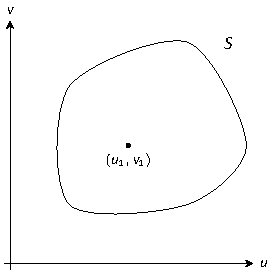
\includegraphics[align=c]{figures/fig13_jacobian_transformation_a} & 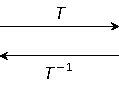
\includegraphics[align=c]{figures/fig13_jacobian_transformation_c} & 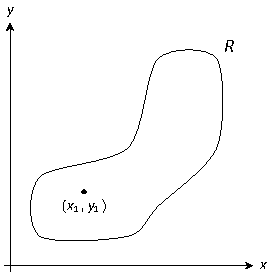
\includegraphics[align=c]{figures/fig13_jacobian_transformation_b}
	\end{tabular}
	\captionsetup{type=figure}%
	\caption{Visualization of the transformation $T$.}
	\label{fig:transformation}
\end{minipage}
\\
\vskip10pt
% further adjusting figure count
\addtocounter{figure}{-2}

\example{ex_transform_box}{Transforming a Rectangle}{
	Consider the tranformation $T(u,v)$ defined by
	\begin{align*}
		x &= u^2\\
		y &= u + v.
	\end{align*}
	Let $S$ be the rectangular region in the $uv$-plane bounded by the lines 
	\[
		u=1, u=2, v=0, \text{ and } v=6
	\]
	shown in figure~.  Described the transformed region $R$ in the $xy$-plane.}
{We first consider the bottom side of the rectangle given by $v=0$ and $1 \leq u \leq 2.$  Using the transformation $T$, we have $x = u^2$ for $1 \leq u \leq 2$ and $y=u + 0.$ Thus, the base of the rectangle in the $uv$-plane transforms into the curve $y = \sqrt{x}$ for $1 \leq x \leq 4$ in the $xy$-plane.
}





%\printexercises{exercises/13_06_exercises}